\section{Unions und enums}


\subsection{enum}

\begin{frame}[fragile]{Definition}
	\begin{block}{Enumeration declarations (Standard, 7.2)}
		\begin{itemize}
			\item Eine \verb|enum| ist eine Aufzählung (enumeration) von benannten Konstanten, den \emph{enumerators}.
			\item Eine \verb|enum| ist ein eigenständiger Typ.
			\item Die Namen der Konstanten liegen auf \emph{der selben Ebene} wie die \verb|enum| selbst -- \alert{sie sind nicht geschachtelt in die enum!}
		\end{itemize}
	\end{block}
	
	\pause
	\footnotesize
	
	\begin{block}{Syntax}
		\lstinputlisting[language=C++, linerange={1-6}, numbers=left, numberstyle=\tiny\color{gray}, tabsize=6, xleftmargin=2em]{cpp-code/enum.cpp}
	\end{block}
\end{frame}

\begin{frame}{Wert eines enumerators}
	enums werden oft als Ersatz für Ganzzahl-Konstanten (integer numbers) verwendet
	
	ABER: Das ist so nicht ganz korrekt und kann zu Fehlern führen!
	
	\pause
	
	\begin{block}{Wert eines enumerators}
		Normalfall:
		\begin{itemize}
			\item der erste enumerator hat den Wert 0
			\item der enumerator n+1 hat einen um 1 größeren Wert als der des enumerators n
		\end{itemize}
		
		\pause
		
		Manuelles eingreifen: Explizites zuweisen eines Wertes an einen enumerator
		
		\footnotesize
		\lstinputlisting[language=C++, linerange={8-11}, numbers=left, numberstyle=\tiny\color{gray}, tabsize=6, xleftmargin=2em]{cpp-code/enum.cpp}
	\end{block}
\end{frame}

\begin{frame}[fragile]{Integral promotion}
	\begin{block}{Underlying type (Standard, 7.2:5)}
		\begin{itemize}
			\item Der \emph{zugrunde liegende Typ} einer enum ist ein Ganzzahl-Typ, der jeden enumerator-Werte dieser enum repräsentieren kann.
			\item Der underlying type soll nicht größer sein als \verb|int|, es sei denn, \verb|int| reicht nicht aus.
		\end{itemize}
	\end{block}
	
	\pause
	
	\begin{block}{Integral promotion of enumerators (Standard, 4.5, 7.2:8)}
		\begin{itemize}
			\item Der Wert enumerators wird wo nötig zu einem Ganzzahl-Typ umgewandelt.
			\item Der Ganzzahl-Typ ist der erste aus folgender Liste, der alle Werte des underlying type repräsentieren kann: \verb|int|, \verb|unsigned int|, \verb|long|, \verb|unsigned long|
		\end{itemize}
	\end{block}
\end{frame}

\begin{frame}{Integral promotion: Beispiel}
	\begin{block}{Beispiel}
		\footnotesize
		
		\lstinputlisting[language=C++, linerange={13-16}, numbers=left, numberstyle=\tiny\color{gray}, tabsize=6, xleftmargin=2em]{cpp-code/enum.cpp}
	\end{block}
	
	\pause
	
	\begin{block}{Typsicherheit}
		\footnotesize
		
		\begin{columns}[t]
			\column{0.575\textwidth}
			\lstinputlisting[language=C++, linerange={1-2, 8-11}, numbers=left, numberstyle=\tiny\color{gray}, tabsize=6, xleftmargin=2em]{cpp-code/enum.cpp}
			
			\column{0.425\textwidth}
			\lstinputlisting[language=C++, linerange={23-29}, numbers=left, numberstyle=\tiny\color{gray}, tabsize=6, xleftmargin=2em]{cpp-code/enum.cpp}
		\end{columns}
	\end{block}
\end{frame}

\begin{frame}{Umgekehrter Weg: conversion}
	\begin{block}{Umgekehrter Weg: Conversion (Standard, 7.2:9)}
		\begin{itemize}[<+->]
			\item Eine Ganzzahl und ein enumerator einer anderen enum kann \emph{explizit} zu einem enumerator \emph{konvertiert} werden.
			\item Der entstehende enumerator hat denselben Wert wie das, was konvertiert wurde -- wenn es einen enumerator mit solchem Wert in der enum gibt.
			\item Ansonsten ist das Resultat \alert{undefiniert!}
		\end{itemize}
	\end{block}
	
	\uncover<+->
	{
		\begin{block}{Beispiel}
			\footnotesize
			
			\lstinputlisting[language=C++, linerange={18-21}, numbers=left, numberstyle=\tiny\color{gray}, tabsize=6, xleftmargin=2em]{cpp-code/enum.cpp}
		\end{block}
	}
\end{frame}

\begin{frame}[fragile]{Hinweise}
	\begin{itemize}
		\item Der underlying type ist \emph{nicht} immer \verb|int|!
		\item Der underlying type ist abhängig vom Compiler und der target platform!
		\item enums sind eigene Typen, aber sehr Typ-unsicher aufgrund der integral promotion
		\item enumerator-Namen werden nicht in die enum geschachtelt
	\end{itemize}
\end{frame}



\subsection{union}

\begin{frame}[fragile]{Was ist eine union?}
	\begin{itemize}
		\item Bekannt: \verb|class| und \verb|struct|
		\begin{itemize}
			\item Fassen Daten (Member) und Methoden zusammen
			\item Das ganze ist (mehr als) die Summe seiner Teile
		\end{itemize}
		\pause
		\item Neu: \verb|union|
		\begin{itemize}
			\item NICHT die Summe aller Teile, KEIN Aggregat
			\item Alle deklarierten Member landen an der gleichen Stelle im Speicher
			\item Ein Union kann Daten verschiedenen Typs aufnehmen
			\item Aber zu jedem Zeitpunkt nur von einem Typ
			\item Nutzung wie bei \verb|class| und \verb|struct|: \verb|myUnion.foo = 42|
			\item Möglich: Methoden, \verb|private, protected, public|, Konstruktoren und Destruktoren
			\item Verboten: Jede Form von Vererbung
		\end{itemize}
	\end{itemize}
\end{frame}

\begin{frame}[fragile]{Unions: Vergleich mit Structs}
	\begin{columns}
		\column{.4\textwidth}
			\lstinputlisting[language=C++]{cpp-code/structunion.cpp}
			
		\column{.6\textwidth}
			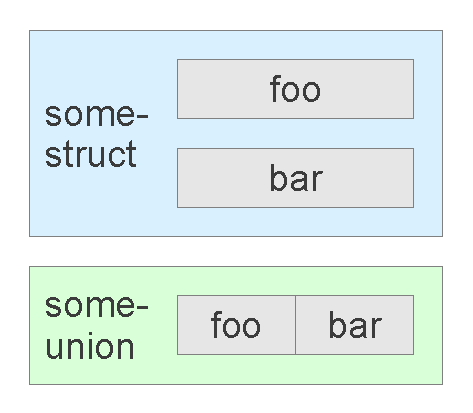
\includegraphics[width=\linewidth]{images/structunion.pdf}
	\end{columns}
\end{frame}

\begin{frame}[fragile]{Unions: Motivation}
	\begin{itemize}
		\item Ursprung: Plain old C, Speicherung verschiedener Typen in einer Variablen
		\begin{itemize}
			\item \enquote{Polymorphismus für Arme}
		\end{itemize}
		\pause
		\item In C++: Auch nur ein Container für verschiedene Typen \dots
		\pause
		\item Type Punning: \verb|foo_t| rein, \verb|bar_t| raus
		\begin{itemize}
			\item Wird NICHT vom Standard gedeckt!
			\item Compilerabhängig
		\end{itemize}
	\end{itemize}
\end{frame}

\begin{frame}[fragile]{Anonyme Unions}
	\begin{itemize}
		\item Unions die selbst nicht in Erscheinung treten/transparent sind
	\end{itemize}
	
	\footnotesize
	
	\begin{columns}[t]
		\column{.45\textwidth}
			\lstinputlisting[language=C++, linerange={1-10}, numbers=left, numberstyle=\tiny\color{gray}, tabsize=6]{cpp-code/anonymous.cpp}
			
		\column{.45\textwidth}
			\lstinputlisting[language=C++, linerange=12, numbers=left, numberstyle=\tiny\color{gray}, tabsize=6]{cpp-code/anonymous.cpp}
	\end{columns}
\end{frame}

\begin{frame}[fragile]{Unions: Anwendungsbeispiel Variant}
	\lstinputlisting[language=C++]{cpp-code/variant.cpp}
\end{frame}

